\documentclass[12pt,letterpaper]{article}

\usepackage[utf8]{inputenc}
\usepackage[spanish]{babel}
\usepackage{times}
\usepackage[left=3cm,top=2.5cm,bottom=2.5cm,right=2.5cm]{geometry}
\usepackage{graphicx}


\begin{document}
\begin{figure}[h!]
\centering
\paragraph{UNIVERSIDAD POLITECNICA DE LA ZONA METROPOLITANA DE GUADALAJARA}
\

\

\includegraphics[scale=0.8]{Upzmg.png} 
\end{figure}
\begin{center}
\textbf{\LARGE Practica 9}\\
\end{center}
\begin{center}
\textbf{\LARGE EV\_ 3\_ 1\_ Diagrama\_ eléctrico\_ de\_ la\_ interfaz\_ de\_ potencia.}
\end{center}


\large{Integrantes:}\\
\large{Guzman Vazquez Jaime Alan.\\
Perez de Alba Santiago Eduardo.\\
Romero Jauregui Osvaldo.\\
Cabrera Gutierrez Raul.\\
Gutierrez Olivares Rogelio.\\
Rodriguez Lopez Francisco Javier.\\

Fecha: 10 de Noviembre del 2019.\\

Curso: Sep-Dic 2019.\\

Carrera: Ingenieria en Mecaronica.\\

Docente: Moran Garabito Carlos Enrique.\\}

\newpage

\section{Objetivo:}
Como tal, el objetivo general de esta penúltima practica consistía en lograr disminuir o aumentar el voltaje de salida comparado con el de entrada dependiendo cuál de los 3 circuitos se armaría. 
\section{Materiales}
\begin{itemize}
\item Baterias de 1.5v.
\item Bobinas de 106 vueltas y 82 vueltas.
\item Capacitores (100uF a 25v, 10uF a 50 v, 220pF a 25v).
\item Fuente de 12v.
\item Mosfet (IRF640N).
\item Resistencias (47 ohm, 68 ohm, 220 ohm).
\item Transistor Tip31c.
\item Transformador de pulsos o bobina con doble campo magnetico.
\item Protoboard
\item Transistor TIP41C
\item Diodos LED
\item Pila 2.5 V
\end{itemize}
\section{Procedimiento:}
Siguiendo el diagrama dado por el maestro, se armó el circuito en nuestra protoboard, considerando cada una de las conexiones de los componentes.

Para la realización de esta practica, el docente, estableció tres diagramas, los cuales cada uno consistía en una tarea diferente, a partir del acomodo y generación del calculo correspondiente, para el sistema del campo magnético y como esto se establece de mejor forma, en un enrollamiento de cobre, el cual genera entre mas vueltas un campo magnético mayor, y a ello, un sistema de disminución o duplicación de voltaje y corriente, así también como la potencia trabajada, en cada parte del sistema a trabajar, en este caso, siendo cada uno de ellos, diferente al otro, pero en reflejo de ello igual, así que esta parte puede confundir un poco, el para que de estos acomodos, si en su observación se reflejan iguales, y la utilización de los mismos, componentes, y es ahí cuando entra el acomodo que se da a cada uno de estos, ya que si por una parte el campo magnético, se genera de una parte al principio este, hará que la potencia disipada, incremente el voltaje y de ello la potencia, pero sin embargo, otra parte, pueda hacer que la bobina, se encuentre después del inicio, lo que hace que el campo magnético generado, sea este menor o mayor, se refleje en la disminución del voltaje y potencia requerida.Tal y como se muestra en los diagramas establecidos.\\

\subsection{Circuito A:}
\begin{figure}[h!]
\centering
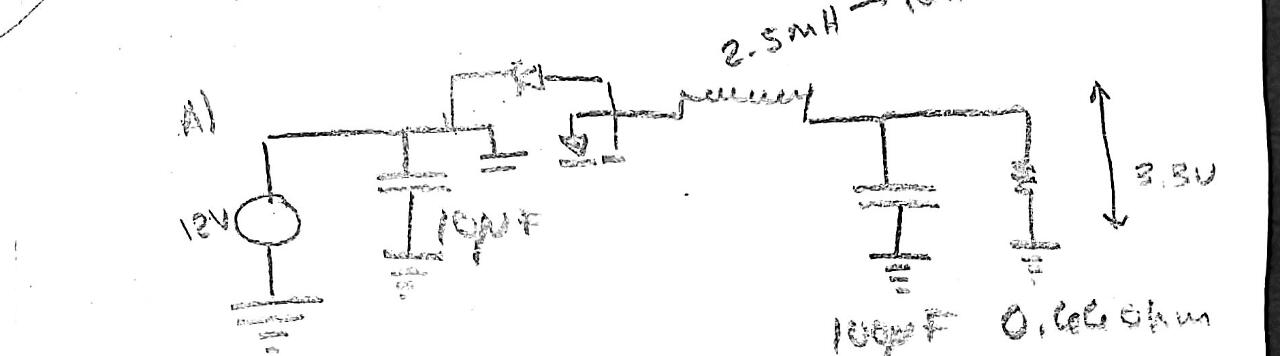
\includegraphics[width=11cm]{esquema1.jpeg}
\caption{Diagrama Disminución de voltaje }
\end{figure}

En el primer esquemático, se tiene como control a un Mosfet, el cual nos ayuda, desde su integrado de un diodo zener, el cual rectifica de mejor forma, la entrada del voltaje de 12v, antes de ello, esta puesto un capacitor de 10uF, esto para que al momento de llegar al Mosfet, este no llegue de lleno a los 12v, sino que se deteriore un poco, desde este punto la entrada del voltaje puesto. Después de haber colocado, el punto anterior, viene el inductor, puesto en marcha, como la parte importante de este esquema, esta tiene que generar un campo magnético de 2.5mH, el cual ayuda a que este circuito, sea de disminución de voltaje, respecto a la colocación en la que se encuentra, el inductor, y cuanto es el campo magnético que genera este, al estar excitado.\\

A ello se le coloca de salida, un condensador de mayores Faradios, ya que al ser puesto de mayor Faradio que el primero, este regula de mejor forma el voltaje directo, haciendo mas lineal, el voltaje de salida, y en su puesta a ello, una resistencia de muy pocos ohmios, ya que si le agregáramos mas ohm, este recibiría el puesto mas grande de saturación de voltaje y corriente, y en ello, el voltaje no disminuiría, sino que simplemente lo saturaría, es por eso que se coloca, una resistencia tan baja como lo es la de 0.66 ohm. En este caso, no se dispuso de una resistencia tan baja por lo que se construyo una , la mas baja que se pudo realizar, quedando en puesta 4 resistencias de 68 ohm en paralelo generando una salida de saturación de 17 ohm, respecto a esta salida, el voltaje de salida, nos da como generación de ello, 3.6v, lo cual al meterle de lleno los 12v, queda por hecho este circuito.
\newpage
\subsection{Circuito B}

\begin{figure}[hbtp]
\centering
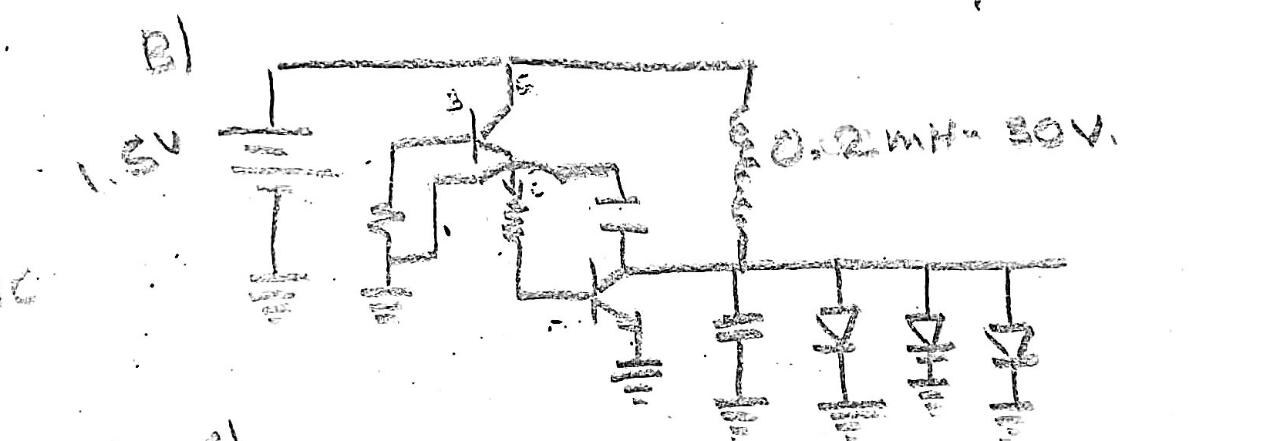
\includegraphics[width=11cm]{esquema2.jpeg}
\caption{Diagrama de elevación de voltaje}
\end{figure}

Este diagrama, tiene como característica, elevar el voltaje, ya sea al doble de su capacidad inicial, o un poco menos de eso, esto ya dependiendo, el colocación que se tenga en esto, en este caso, se tiene como entrada una batería de 1.5v, se estableció este pequeño voltaje, para el encendido de unos leds, como prueba de su elevación, y estancia de ello, su acomodo. En su parte positiva de la batería, se tiene un Tip41c, se utiliza un transistor de alta potencia, ya que la generación de ello, tiene que ser su objetivo, tener a la entrada una potencia baja, pero a la salida, una potencia mayor, y este en su acomodo, puede realizar ese trabajo, se tienen dos, ya que la potencia disipada, en el inductor es menor al del esquemático anterior, ya que este no debe de generar un campo magnético tan grande, sino que solo tiene que inducir lo necesario, para transmitir el voltaje, este es el contrario al transistor, ya que este dobla solo la potencia, y la transimite a partir de la corriente.\\

De ello, tenemos una salida con un condensador, en esta parte se cumple la misma función que en el caso anterior, ya que la onda generada a partir del condensador, es lineal, convirtiendo mas pura la salida de la potencia, haciendo que los 3 leds, puestos con prueba de ello, prendan sin problemas, aunque aquí se genera una complicación, ya que el circuito empieza  a doblar su voltaje, y potencia, cuando es colocada un voltaje de 2.6v, por lo que los 1.5 de la batería, no son suficientes, para la conmutación y doblamiento de la potencia requerida a la salida. Se debe de tener en cuenta, el campo magnético generado, generado por el inductor, ya que si este es muy grande, o en reversión a ello, muy pequeño, generando complicaciones, a la salida de potencia, voltaje y corriente.\\

Al conectar nuestra pila, la entrada es de 2.5 V, nuestros leds logran encender (3), si hacemos la medición de Voltaje de salida, obtendríamos como resultado 3.03V, logrando encender los LEDs.
\subsection{Circuito C:}
\begin{center}
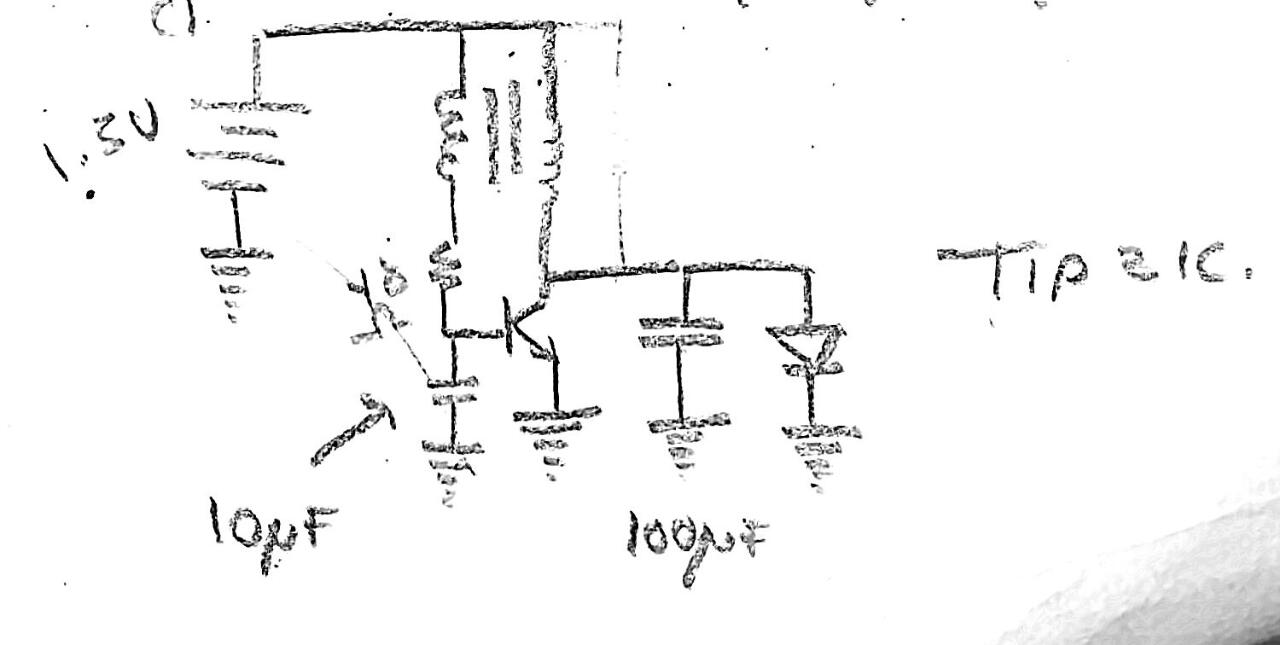
\includegraphics[width=9cm]{esquema3.jpeg}
\end{center}

Este ultimo circuito, tiene como objetivo elevar el voltaje, pero en este caso, se tvo complicaciones, las cuales se tuvieron en cuenta, ya que a la entrada se tiene una batería de 1.5v, generado como en el esquematico anterior un duplicador del voltaje de inicio, en relevancia a ello, y la colocación, que se tiene en el esquemático, en donde se encuetra un transformador, de la entrada de ellos, al positivo de la batería, en este caso, se tuvo a la disposición un transformador y un solenoide de doble enrollamiento, en este caso, para suplementar al transformador, se tiene como perspectiva, que cualquiera de los dos componentes, se comporten de la misma forma, ya que el tornillo, al tener un enrollamiento, y se pone encima de ello, otro enrrollamiento, con un calibre menor de cobre, se tiene que tener en constancia un transformador, ya que tiene en si, dos campos magnéticos, para generar.\\

En una terminal del campo magnético 2, se coloca a ello, el conector del transistor Tip31c, ya que este transistor al igual que el anterior, es de alta potencia, al hacer esto, se espera que también duplique el voltaje de entrada, y por otra parte, se tiene a la terminal del campo magnético 1, conectado a una resistencia de 220 ohm, y de ello, la conexión a la base, se coloca una resistencia en este punto, para la saturación de voltaje disipado por el inductor, y de ello el emisor del transistor se sitúa en tierra, así como en los casos anteriores, se pone un condensador a la salida de voltaje, para que esta realice lo mismo que seria, tener el voltaje de manera mas lineal, que al principio, y a ello, un diodo Led, para el señalamiento de la duplicación de voltaje, pero en este caso, hubo al igual que en el anterior fallas, ya que en ocasión a duplicar, resta a la mitad, el voltaje que tenemos a la entrada, siendo este circuito, restador, para así tener a la salida, un voltaje de menor potencia y menor voltaje, pero con la misma corriente de entrada, dejando ver, que la disipación de los campos magnéticos, es mucha, y de ello la disminución de voltaje.\\

Nota: Todas las salidas van a tierra, esto para generar la comunicación con la segunda parta de cada uno de los componentes a usar.

\section{Resultados:}

\subsection{Circuito A}
Se tiene que generar y armar un inductor, con un campo magnético de 2.5mH, por lo que la generación del solenoide, queda establecida por el un calculo, el cual nos deja ver las vueltas que se les tiene que dar, para la generación de este campo magnético. \\

Formula utilizada:\\
$$ n=\sqrt{\frac{L*Cx10^{8}}{1,256 x S}} $$

Obteniendo, los datos a partir del tornillo utilizado, queda como:\\
$$ n=\sqrt{\frac{2.5mH*0.014x10^{8}}{1,256 * 1.5x10^{-4}}}= 106 vueltas. $$

La superficie, es $ \pi $ por radio al cuadrado, por lo que la generación de esto, se saca, a partir de datos obtenidos.\\
$$ S=\pi * r^{2} $$
\newpage
Quedando como:\\

$$ S=\pi * \frac{0.014m}{4}^{2}= 1.5x10^{-4} $$

Teniendo en cuenta las vueltas que se le darán al solenoide, este sera el suficiente, para generar el campo magnético requerido, a partir del cobre que se tenga. Dejando una disminución de 3.6v.\\

\begin{center}
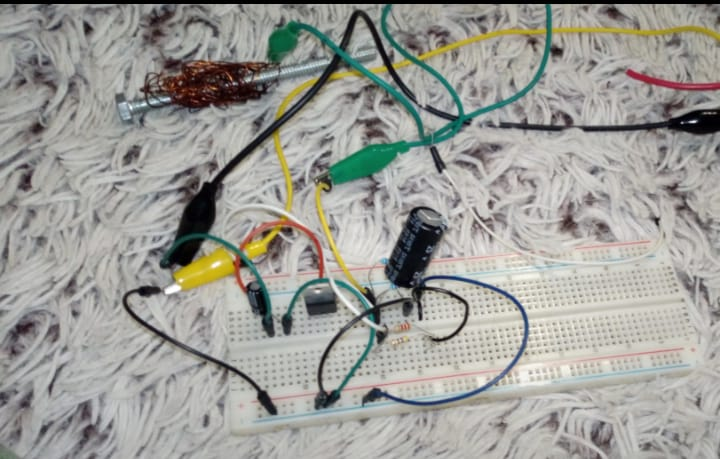
\includegraphics[width=10cm]{resul1.jpeg} 
\end{center}

\subsection{Circuito B}
En este caso, se establecen ya las vueltas que se tienen que dar, pero en este caso, el campo magnético generado con 30 vueltas, es muy poco, por lo que queda establecido de la siguiente forma:\\
$$ L=1,256* \frac{S * n^{2}}{C}x10^{-8} $$

Simplificando datos:\\
$$ L=1,256* \frac{1.5x10^{-4} * 30^{2}}{0.014m}x10^{-8}= 0.4mH $$

En este caso, es muy poco el campo magnético generado, por lo que se queda establecido, que las vueltas deberían de ser mas, para un campo magnético mayor:\\
$$ n=\sqrt{\frac{1.5mH*0.014x10^{8}}{1,256 * 1.5x10^{-4}}}= 82 vueltas. $$

Generando así el campo magnético requerido, para la duplicación de voltaje, y el encendido de los Led.\\

\begin{center}
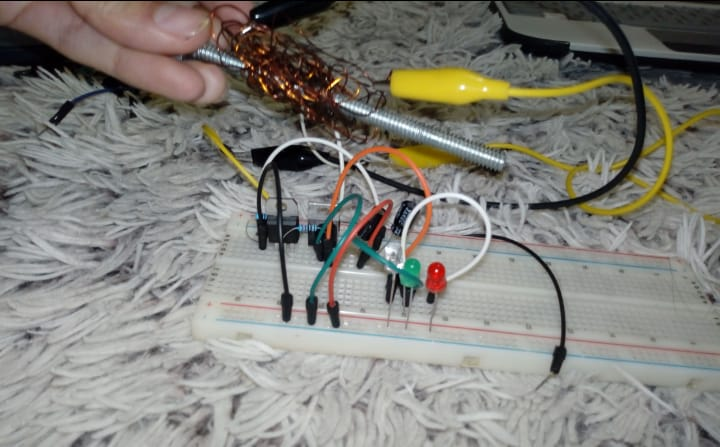
\includegraphics[width=8cm]{resul2.jpeg} 
\end{center}

\subsection{Circuito C}

El calculo, para este caso, es el mismo que en el caso 1, simplemente a este se le añade, doble embobinado, para así poder tener en cuenta el transformador que se requiere, los resultados lanzados n este caso, dan por generación un campo magnético de 5mH, por lo que el campo magnético es mucho mayor a los dos casos anteriores, y de ello, la generación en su relación, con la comunicación de los componentes y su transmisión de ellos.

\begin{center}
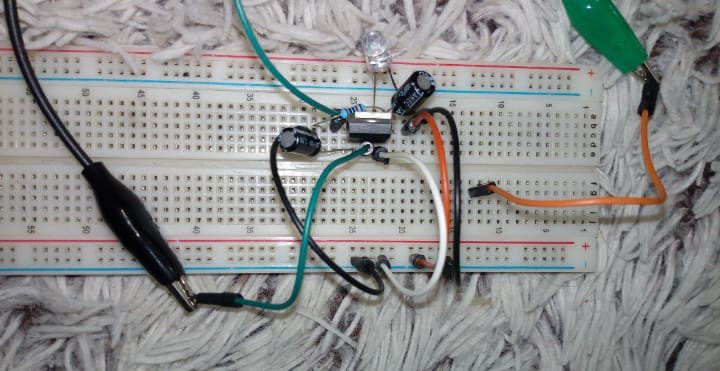
\includegraphics[width=9cm]{resul3.jpeg} 
\end{center}

\newpage
\section{Conclusiones:}
\begin{itemize}
\item \textbf{Jaime Guzman.}\\
Esta aplicacion dada por estos tres circuitos es muy relevante para el mundo de la electrónica debido a que permite a dispositivos de bajo consumo o de voltaje bajo a convivir con dispositivos de voltaje alto debido a esta podría llamarse control de voltaje.\\\\
Este tipo de circuitos tienen un gran grado de libertad en cuestión de aplicaciones practicas debido a la gran variedad en el consumo de energía de los diferentes dispositivos así como las diferentes propiedades de cada uno los hacen muy útiles y versátiles para las diferentes implementaciones que se requieran en los diferentes proyectos en los que se quieran ver implementados.
\item \textbf {Santiago Perez}\\
Durante la realización de la practica se pudo poner a prueba distintos circuitos como lo fueron un Buck, Un Boost y un conversor de CA-CD, se pudo poner a prueba conocimiento previos para la correcta función, donde se puede observar que el circuito del Boost pudimos obtener incrementos de voltajes en la salida demasiados elevados(+70v) aunque tuviéramos una entrada muy pequeña de voltaje (12), mientras que el buck se podía observar un disminución de nuestro voltaje de entrada por mitad, al momento de aplicarlo en una fuente con una conversión de CA-CD e implementarle el boost obtuvimos un aumento de voltaje regulable y mucho mas estable que un boost simple que puede llegar a ser muy inestable.
\item \textbf{Rogelio Gutierrez}\\
Esta practica ayudó a comprender de una manera mas claro y en forma el funcionamiento de las tensiones dentro de los circuitos aportando el conocimiento de poder cambiarlas según sea la necesidad del circuito lo que nos brindara un gran apoyo en próximos trabajos y proyectos.
\item \textbf{Raul Cabrera:}\\
Los materiales en interfaces de potencia son lo que requieren las comunicación para sistemas de corriente en transpiración a ello, generado por campos magnéticos, los cuales pueden ser ejecutados en sistemas mas complejos y de mayor estructura, para así tener en cuenta cada etapa que se estuvo viendo en estas dos practicas, tanto en la 8 con su conmutación en estado convertidor, hasta la 9, con un estado de control mejor, y de mayor forma a lo requerido para el movimiento y dinámica de los objetos que se requiere menos o mas potencia disipada en un equipamiento de mejor forma.
\item \textbf{Osvaldo Romero:}\\
Durante la realización de esta practica se obtuvieron varios problemas para conseguir el resultado deseado. Desde el no conseguir el valor de voltaje deseado, hasta no conseguir el encendido de nuestros componentes. Tomando en cuenta conocimientos previamente adquiridos, se logro determinar la causa de la falla y así poder solucionarla.
\item \textbf{Francisco Javier}\\
La generación de acomodos, arreglos, dentro de lo que es el voltaje y la conmutación entre los componentes, que manejan la potencia, son de suma importancia, a la hora de trabajar, con todo esto, siendo cada relación, algo similar y relevante a lo que se utiliza en un  sistema mas avanzado como lo seria un convertidor de corriente alterna a corriente continua, para así tener en claro que tenemos que hacer, y como se debe de hacer, para el buen control y el buen resultado de ello, y de alguna u otra forma, ver como la inductancia que se pueda tener, en estos circuitos, puede ser expandida en sistemas mas complejos.\\

Para asi poder tener, algo generado en estas practicas, y que se pueda realizar en un proyecto a futuro, observando y analizando, interfaces de potencia, para así poder tener en estancia el correcto uso de arreglos eléctricos, y electrónicos, que en su mayor relevancia disminuyan o dupliquen, la entrada a la potencia y corriente requerida por los objetos a ver, y como estos, pueden ser de gran utilidad, al tener la misma corriente que al inicio, o en algunos casos, duplicarla, para nuestro beneficio.\\

\end{itemize}


\textbf{\Large Referencias:}\\
Carlos Enrique Móran Garabito, Sistemas Electrónicos de Interfaz, Curso: Sep-Dic 2019 c, Diagrama eléctrico de la interfaz de potencia.

\end{document}